\section{Experiments and Analysis}
\label{sec:experiments}
\vspace{-1mm}
%\subsection{Experimental Setups}
%\label{subsec:setup}

%%
\textbf{Baselines.}
%
We compare \sysname against three groups of methods: (1) Vanilla SVD and state-of-the-art SVD-based LLM compression methods: FWSVD~\citep{DBLP:conf/iclr/HsuHCLSJ22}, ASVD~\citep{DBLP:journals/corr/abs-2312-05821} (Section~\ref{subsec:overall_performance}) and FLAP (\cref{appendix:flap_comparison}).
%
(2) Other types of LLM compression methods. These include three state-of-the-art pruning-based LLM compression methods: LLM-Pruner~\citep{DBLP:conf/nips/MaFW23}, SliceGPT~\citep{DBLP:conf/iclr/AshkboosCNHH24}, and BlockPruner~\citep{DBLP:journals/corr/abs-2406-10594}, and three state-of-the-art quantization-based LLM compression methods: PB-LLM~\citep{DBLP:conf/iclr/YuanSD24}, BiLLM~\citep{DBLP:conf/icml/HuangLQLZ0M024}, and OneBit~\citep{DBLP:conf/nips/Xu0YWZLLC24} (Section~\ref{subsection:Comparison_with_other_compression_methods}). 
%
(3) Smaller LLM StableLM-3B~\citep{StableLM-3B-4E1T} pre-trained from scratch (\cref{appendix:pretrained_comparison}).

\textbf{Models and Datasets.} 
%
To demonstrate the generability of \sysname, we evaluate the performance of \sysname on seven models from three different LLM families at three different scales (LLaMA-7B, 13B, 30B, LLaMA2-7B~\citep{DBLP:journals/corr/abs-2307-09288}, OPT-6.7B~\citep{DBLP:journals/corr/abs-2205-01068}, Vicuna-7B~\citep{vicuna2023} and Mistral-7B~\citep{DBLP:journals/corr/abs-2310-06825}) and $10$ datasets including two language modeling datasets (WikiText-2~\citep{DBLP:conf/iclr/MerityX0S17}, and C4~\citep{DBLP:journals/jmlr/RaffelSRLNMZLL20}), six classification datasets (OpenbookQA~\citep{DBLP:conf/emnlp/MihaylovCKS18}, WinoGrande~\citep{DBLP:conf/aaai/SakaguchiBBC20}, HellaSwag~\citep{DBLP:conf/acl/ZellersHBFC19}, Arc\_e~\citep{DBLP:journals/corr/abs-1803-05457}, PIQA~\citep{DBLP:conf/aaai/BiskZLGC20}, MathQA~\citep{DBLP:conf/naacl/AminiGLKCH19}),  and two generation datasets (TruthfulQA~\citep{DBLP:conf/acl/LinHE22} and GSM8K~\citep{DBLP:journals/corr/abs-2110-14168}) with the LM-Evaluation-Harness framework~\citep{eval-harness}.

%
\textbf{Implementation Details.}
%
To ensure a fair comparison, we followed ASVD~\citep{DBLP:journals/corr/abs-2312-05821} to randomly select 256 samples from WikiText-2 as the calibration data. 
We followed the same configuration used in LLM-Pruner~\citep{DBLP:conf/nips/MaFW23} to use Alpaca~\citep{alpaca} dataset with 50K samples for parameter update in \sysname.
% All of our experiments are conducted on NVIDIA A100 GPUs.
The inference efficiency experiment is conducted on both NVIDIA A100 GPU and AMD EPYC 7643 CPU while the other experiments are conducted on NVIDIA A100 GPUs.
%Due to page limit, implementation details are provided in~\cref{appendix:experimental_setup}.

%%Compression Accuracy Analysis
\vspace{-2mm}
\subsection{Comparison with State-of-the-Art SVD-based LLM compression Methods}
\label{subsec:overall_performance}
\vspace{-2mm}
First, we compare the performance of \sysname with state-of-the-art SVD-based LLM compression methods from four aspects: (1) performance under different compression ratios, (2) performance on different LLMs, (3) performance on LLMs with larger scales, and (4) compression speed (\cref{appendix:compression_speed}). 
%
Given that all the SVD-based baselines do not incorporate LoRa fine-tuning, to ensure a fair comparison, we also compare to 
\sysname with truncation-aware data whitening only (denoted as \sysname \texttt{(W)}).

\accuracyTable
\differntllmaccuracyTable
\textbf{Performance under Different Compression Ratios.}
We first evaluate the performance of LLaMA-7B compressed by \sysname, \sysname \texttt{(W)}, and the SVD-based baselines under compression ratios ranging from 20\% to 80\% on all $10$ datasets. 
%
The results are summarized in\cref{tab:dataset_acc}. Both \sysname and \sysname \texttt{(W)} consistently outperform vanilla SVD, FWSVD and ASVD across all the compression ratios. In particular, when the compression ratio is 40\% and above, \sysname reduces the perplexity by more than 99\% on two language modeling datasets and achieves over 400\% higher average accuracy on six classification datasets. More importantly, the results on two generation datasets (TruthfulQA, GSM8K) of all three baselines when compression ratios are 60\% and above are zero, meaning that the compressed LLMs totally lose their generation ability. In contrast, \sysname still outputs good generation even under 80\% compression ratio. 
%
Example contents generated by the compressed LLMs are included in~\cref{sec:appendix_example}.
%
%These results indicate that \sysname is more effective in compressing LLMs for more resource-constrained devices such as smartphones and IoT devices.

%%


\begin{wrapfigure}{r}{0.48\textwidth} % "r" 表示右侧，"0.5\textwidth" 控制宽度
  \centering
  \vspace{-5mm}
  \largellmaccuracyTable
\end{wrapfigure}

\textbf{Performance on Different LLMs.} To examine the generability of \sysname and \sysname \texttt{(W)} across different LLMs, we compare the performance between \sysname and the baselines on four different models from three different LLM families -- OPT-6.7B (OPT family), LLaMA 2-7B (LLaMA family), Mistral-7B (Mistral family), and Vicuna-7B (LLaMA family)  -- under 20\% compression ratio on WikiText-2 and six classification datasets. 
%
As shown in~\cref{tab:different_llm_acc}, both \sysname and \sysname \texttt{(W)} consistently outperform baselines on all four LLMs, and exhibits more stable performance across different LLMs, especially compared to vanilla SVD and FWSVD.

\textbf{Performance on LLMs with Larger Scales.} To examine the generability of \sysname and \sysname \texttt{(W)} on LLMs with larger scales, we compare the performance between \sysname and the baselines on LLaMA-13B and LLaMA-30B under 20\% compression ratio. As shown in~\cref{tab:large_llm_acc}, both \sysname and \sysname \texttt{(W)} consistently outperform vanilla SVD, FWSVD, and ASVD on both model sizes. 


\vspace{-1mm}
\subsection{Inference Efficiency of \sysname }
\label{subsec:inference_speedup}
\vspace{-1mm}
% Next, to illustrate the inference speedup and memory reduction of LLMs compressed by \sysname, we provide theoretical analysis as well as empirical evaluation on real-world hardware.

\textbf{Theoretical Analysis of Inference Efficiency.} Assume \sysname compresses the weight matrix {\small$W \in \mathbb{R}^{d \times n}$} into two low-ranking matrices {\small$W_u' \in \mathbb{R}^{d \times r}, W_v' \in \mathbb{R}^{r \times n}$}. The compression ratio is then calculated as {\small$R_w = 1-\frac{(d+n) r}{d n}$}.

\underline{(1) Compute Complexity Analysis:} Given input {\small$X \in \mathbb{R}^{n \times d}$}, instead of recalculating the full weight matrix {\small$W^{\prime}=W_u' \times W_v'$} and then computing the output {\small$W^{\prime} \times X$}, \sysname calculates the intermediate state {\small$M=W_v' \times X$} and then computes the output {\small$Y=W_u' \times M$}. 
%
In this way, the computation complexity is reduced from {\small$O\left(d^2 n\right)$} to {\small$O\left(d^2 r+r n d\right)$}. 
%
Taking compression ratio {\small$R_w=50\%$} as an example, since {\small$R_w=1 - \frac{(d+n) r}{d n}$}, we have {\small$r=\frac{d n}{2(d+n)}$}. Then the computation complexity is
{\small$O\left(d^2 r+r n d\right)=O(r d(d+n))=O\left(\frac{d^2 n}{2}\right)=\frac{1}{2} O\left(d^2 n\right)$}, which reduces {\small$50\%$}. In general, given any compression ratio $R_w$, the computation complexity is reduced to {\small$1 - R_w$} times of the original.

\begin{figure}[htbp]
 \vspace{-0mm}
     \begin{minipage}{0.98\textwidth}
     \centering
    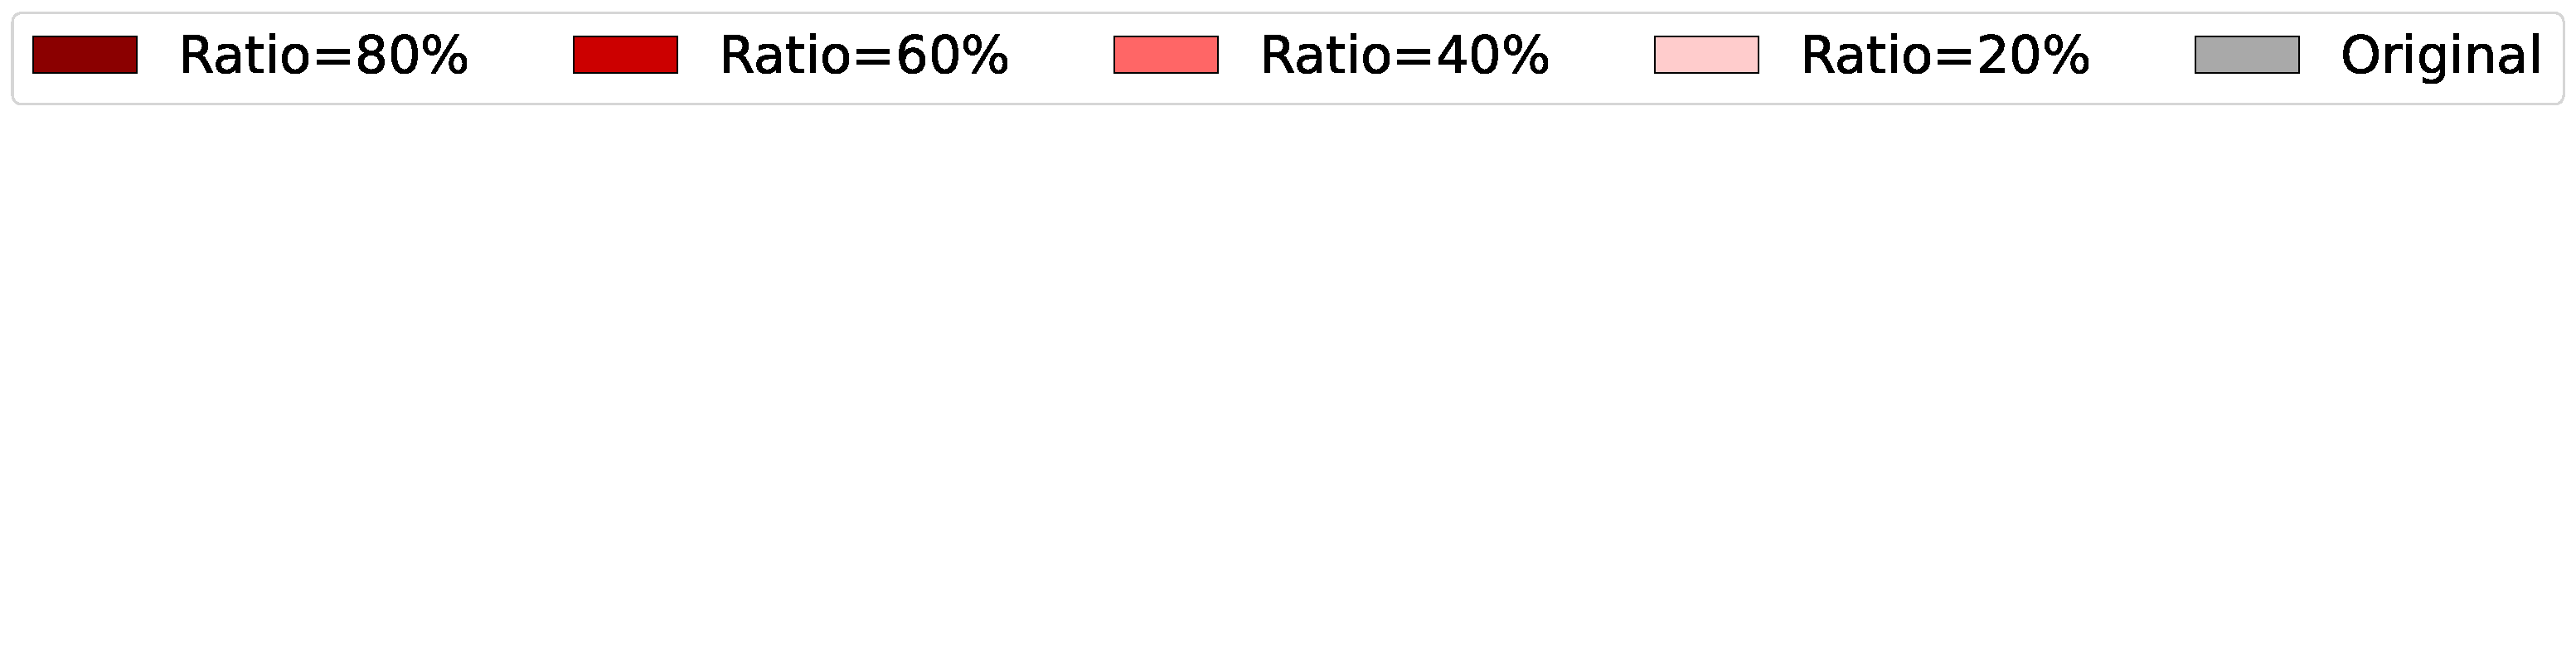
\includegraphics[width=1\linewidth]{Figures/legend.pdf}
     \end{minipage}
     \\
     \begin{minipage}{1\textwidth}
        \subfigure[Varying Batch Size on GPU]{
            \centering
            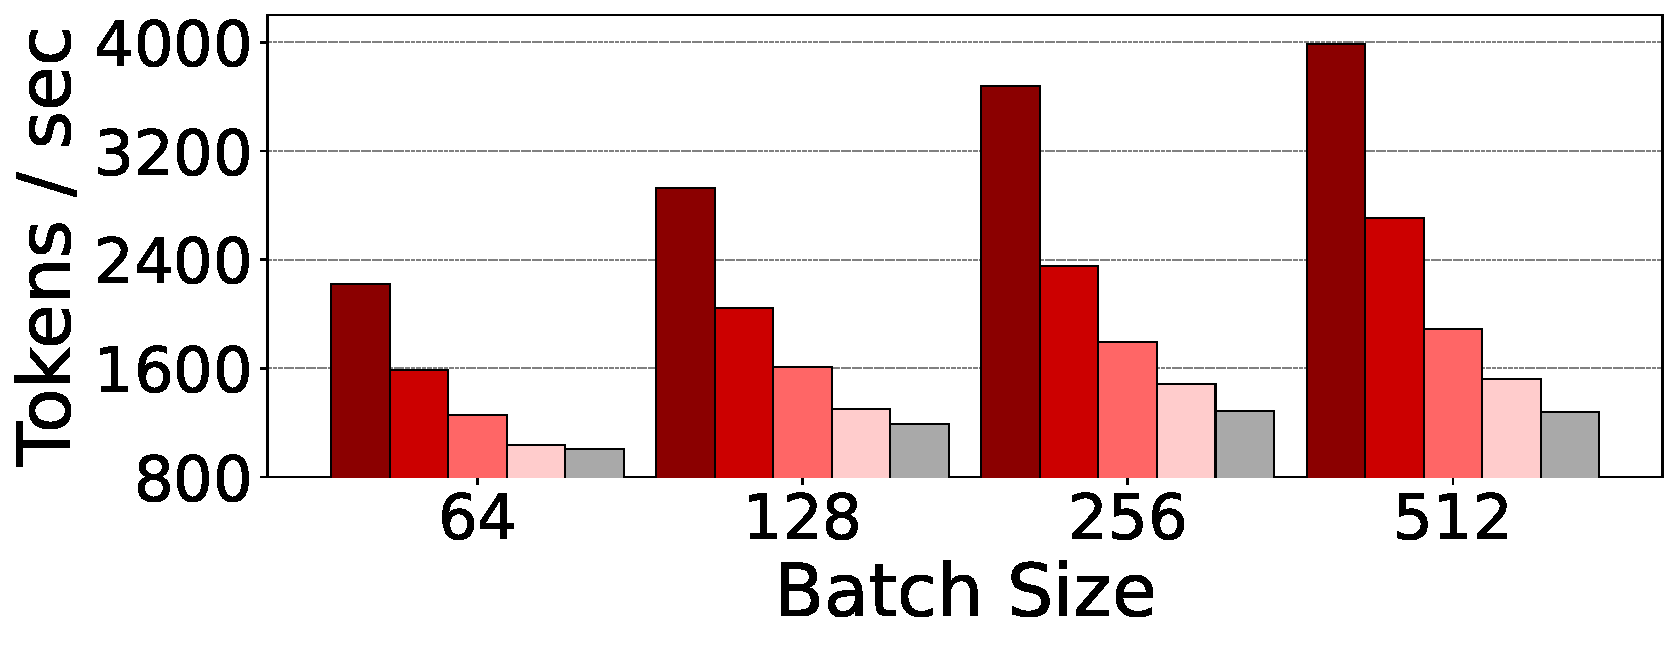
\includegraphics[width=0.48\textwidth]{Figures/eff_bs_gpu.pdf}
            \label{fig:bs_gpu}
            }
        \subfigure[Varying Sequence Length on GPU]{
            \centering
            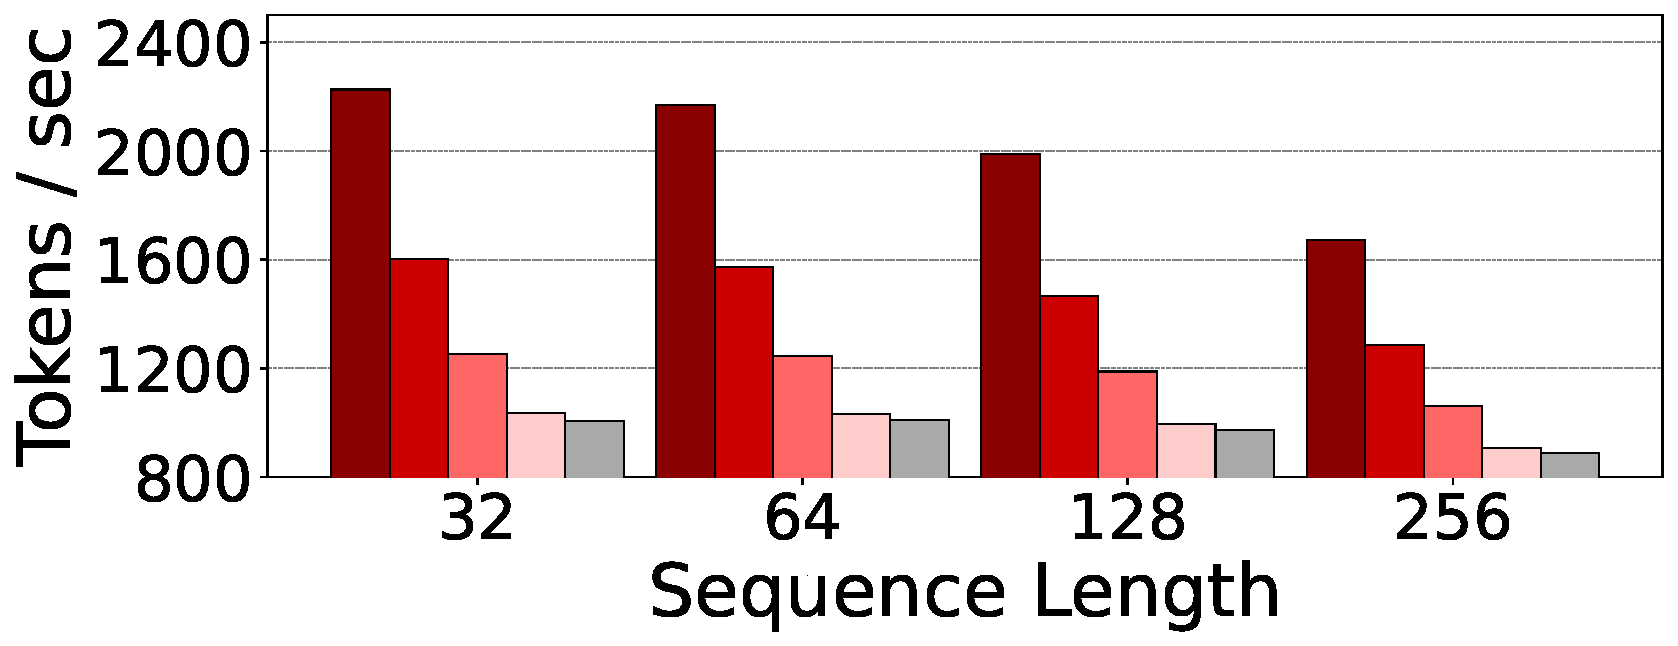
\includegraphics[width=0.48\textwidth]{Figures/eff_sl_gpu.pdf}
            \label{fig:sl_gpu}
            }
        \\
        \subfigure[Varying Batch Size on CPU]{
            \centering
            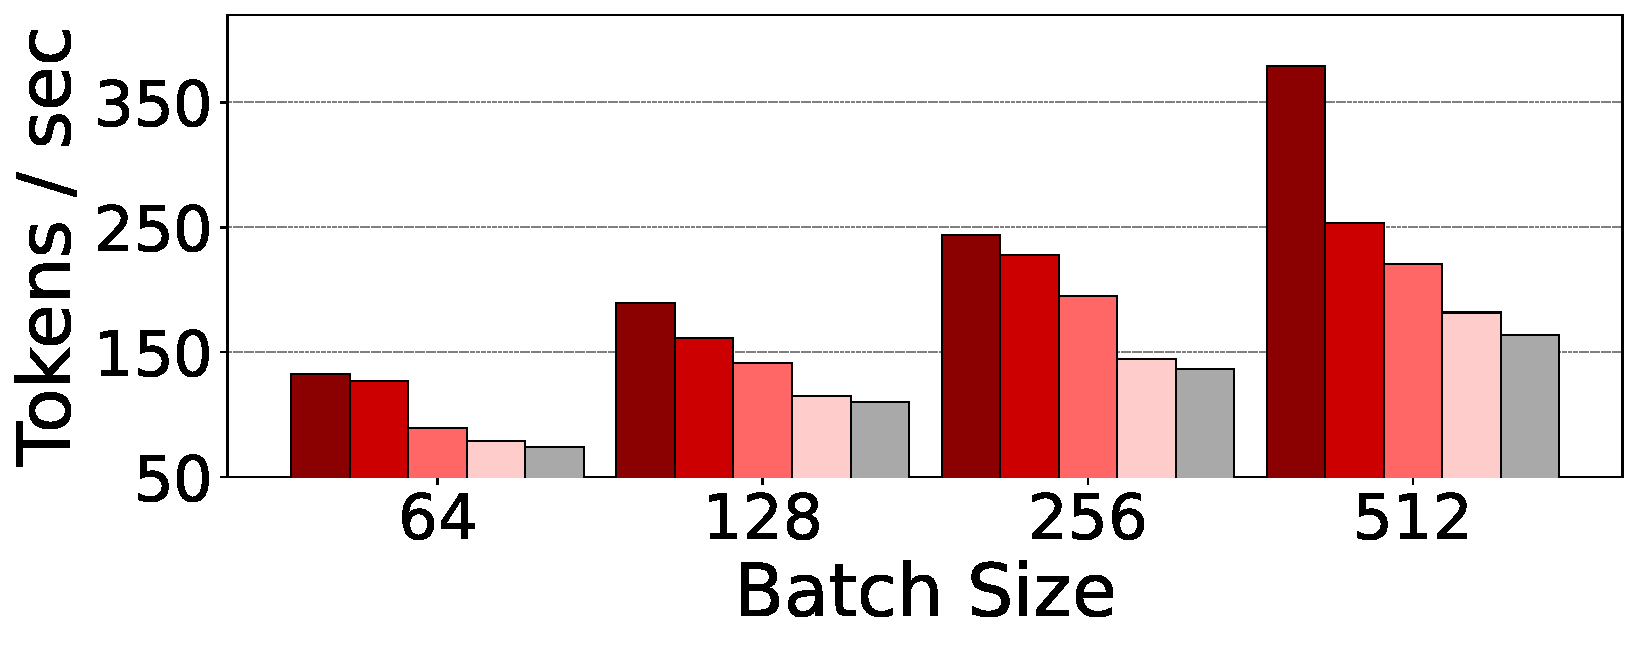
\includegraphics[width=0.48\textwidth]{Figures/eff_bs_cpu.pdf}
            \label{fig:bs_cpu}
            }
        \subfigure[Varying Sequence Length on CPU]{
            \centering
            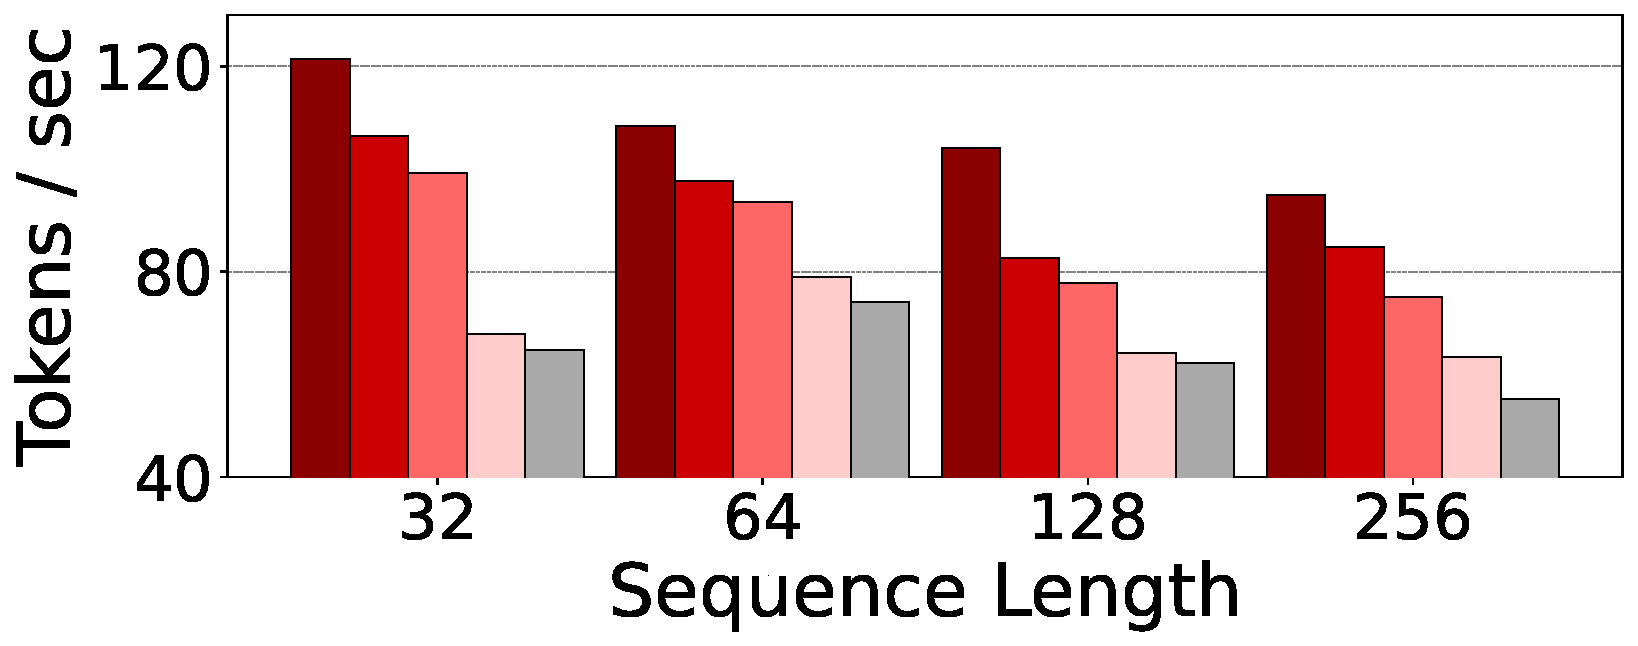
\includegraphics[width=0.48\textwidth]{Figures/eff_sl_cpu.pdf}
            \label{fig:sl_cpu}
            }
        \DeclareGraphicsExtensions.
        \vspace{-2mm}
        \caption{Throughput (tokens/sec) of LLaMA-7B and its compressed version by \sysname under different compression ratios on a single A100 GPU under different batch sizes (a) and different sequence lengths (b) and on a single AMD EPYC 7643 CPU under different batch sizes (c) and different sequence lengths (d). For (a) and (c), sequence length is 32. For (b) and (d), batch size is 64.}
        \vspace{-2mm}
        \label{fig:gpu_throughput}
    \end{minipage}
\end{figure}

\underline{(2) Inference Memory Analysis:} 
%
Since \sysname does not recalculate the full weight $W^{\prime}=W_u' \times W_v'$, the weight memory is reduced to $1 - R_w$ times of the original during inference.
%
As another advantage, \sysname is able to reduce the runtime KV cache memory as well~\citep{DBLP:journals/corr/abs-2406-13035, wan2025meda,DBLP:journals/corr/abs-2409-09808}. Specifically, instead of keeping {\small$W_u' \times W_v' \times X$} in the KV cache, \sysname provides the option to store the intermediate result {\small$M=W_v' \times X$} in the KV cache and recomputes the original key and value states with the decomposed weight matrix {\small$W_u'$} if required. As such, the runtime KV cache is reduced to {\small$\frac{r}{d}= (1 - R_w)\times \frac{d}{n+d}$} times of the original. Moreover, since {\small$W_u'$} is already stored as the weight matrix in the decomposed LLM, the original intermediate state matrix can still be recovered by {\small$W_u'\times M$} without accuracy drop. Therefore, \sysname provides a unified solution that enables \textit{simultaneous} model compression and KV cache compression.
%into a single process. 
% This is different from existing quantization or parameter pruning-based LLM compression methods that need to be combined with other techniques for compressing both weights and KV cache. 


\textbf{Inference Speedup on Hardware.} 
%
To quantify inference speedup achieved by \sysname on real hardware, we measure the numbers of tokens that LLaMA-7B and its compressed version by \sysname generate per second (i.e., throughput) under different batch sizes and sequence lengths on a single NVIDIA A100 GPU and a single AMD EPYC 7643 CPU, respectively. 
%
The results are shown in~\cref{fig:gpu_throughput}. We have three observations. 
%
(1) Under a specific batch size or sequence length, the speedup achieved by \sysname related to the original model increases as the compression ratio increases.
%consistently enhances the token generation speed across all the compression ratios. 
%
(2) Under a specific compression ratio, the speedup  achieved by \sysname related to the original model becomes more significant as the batch size increases or as the sequence length decreases.
%
(3) The above two observations are valid for both GPU and CPU.
%resulting in a maximum speedup of 1.2x on GPU and 1.1x on CPU under 20\% compression ratio, 1.7x on GPU and 1.5x on CPU under 40\% compression ratio, 2.1x on GPU and 1.64x on CPU under 60\% compression ratio, and 3.1x on GPU and 2.3x on CPU under 80\% compression ratio. 
%These results highlight the effectiveness of \sysname in enhancing the inference efficiency of LLMs on real hardware.


\textbf{Inference Memory Reduction on Hardware.} 
% \sysname is able to compress not only LLMs but also the runtime KV cache \textit{at the same time}.
Lastly, we evaluate the inference memory saving, including both weight memory and runtime KV cache memory saving on a single A100 GPU. 
%
Specifically, we measure the peak memory footprint during inference when generating 128 tokens with batch size of 32 using LLaMA-7B compressed by \sysname under different compression ratios w/ and w/o considering KV cache reduction. 
%
The results are illustrated in~\cref{fig:kv} where the memory reduction from the dotted line to the blue bars comes mainly from model weight compression and the memory reduction from the blue bars to the yellow bars comes mainly from KV cache compression. 
%
As shown, both weight memory saving and runtime KV cache memory saving brought by \sysname are near linear to the compression ratio.
%, which aligns with our theoretical analysis. 
%In particular, \sysname is able to save additional 51\% memory from its KV cache under 80\% compression ratio.


\begin{figure}[htbp]
\vspace{-5mm}
    \centering
    \begin{minipage}{0.5\textwidth}
    \centering
    \vspace{4mm}
        \centering
        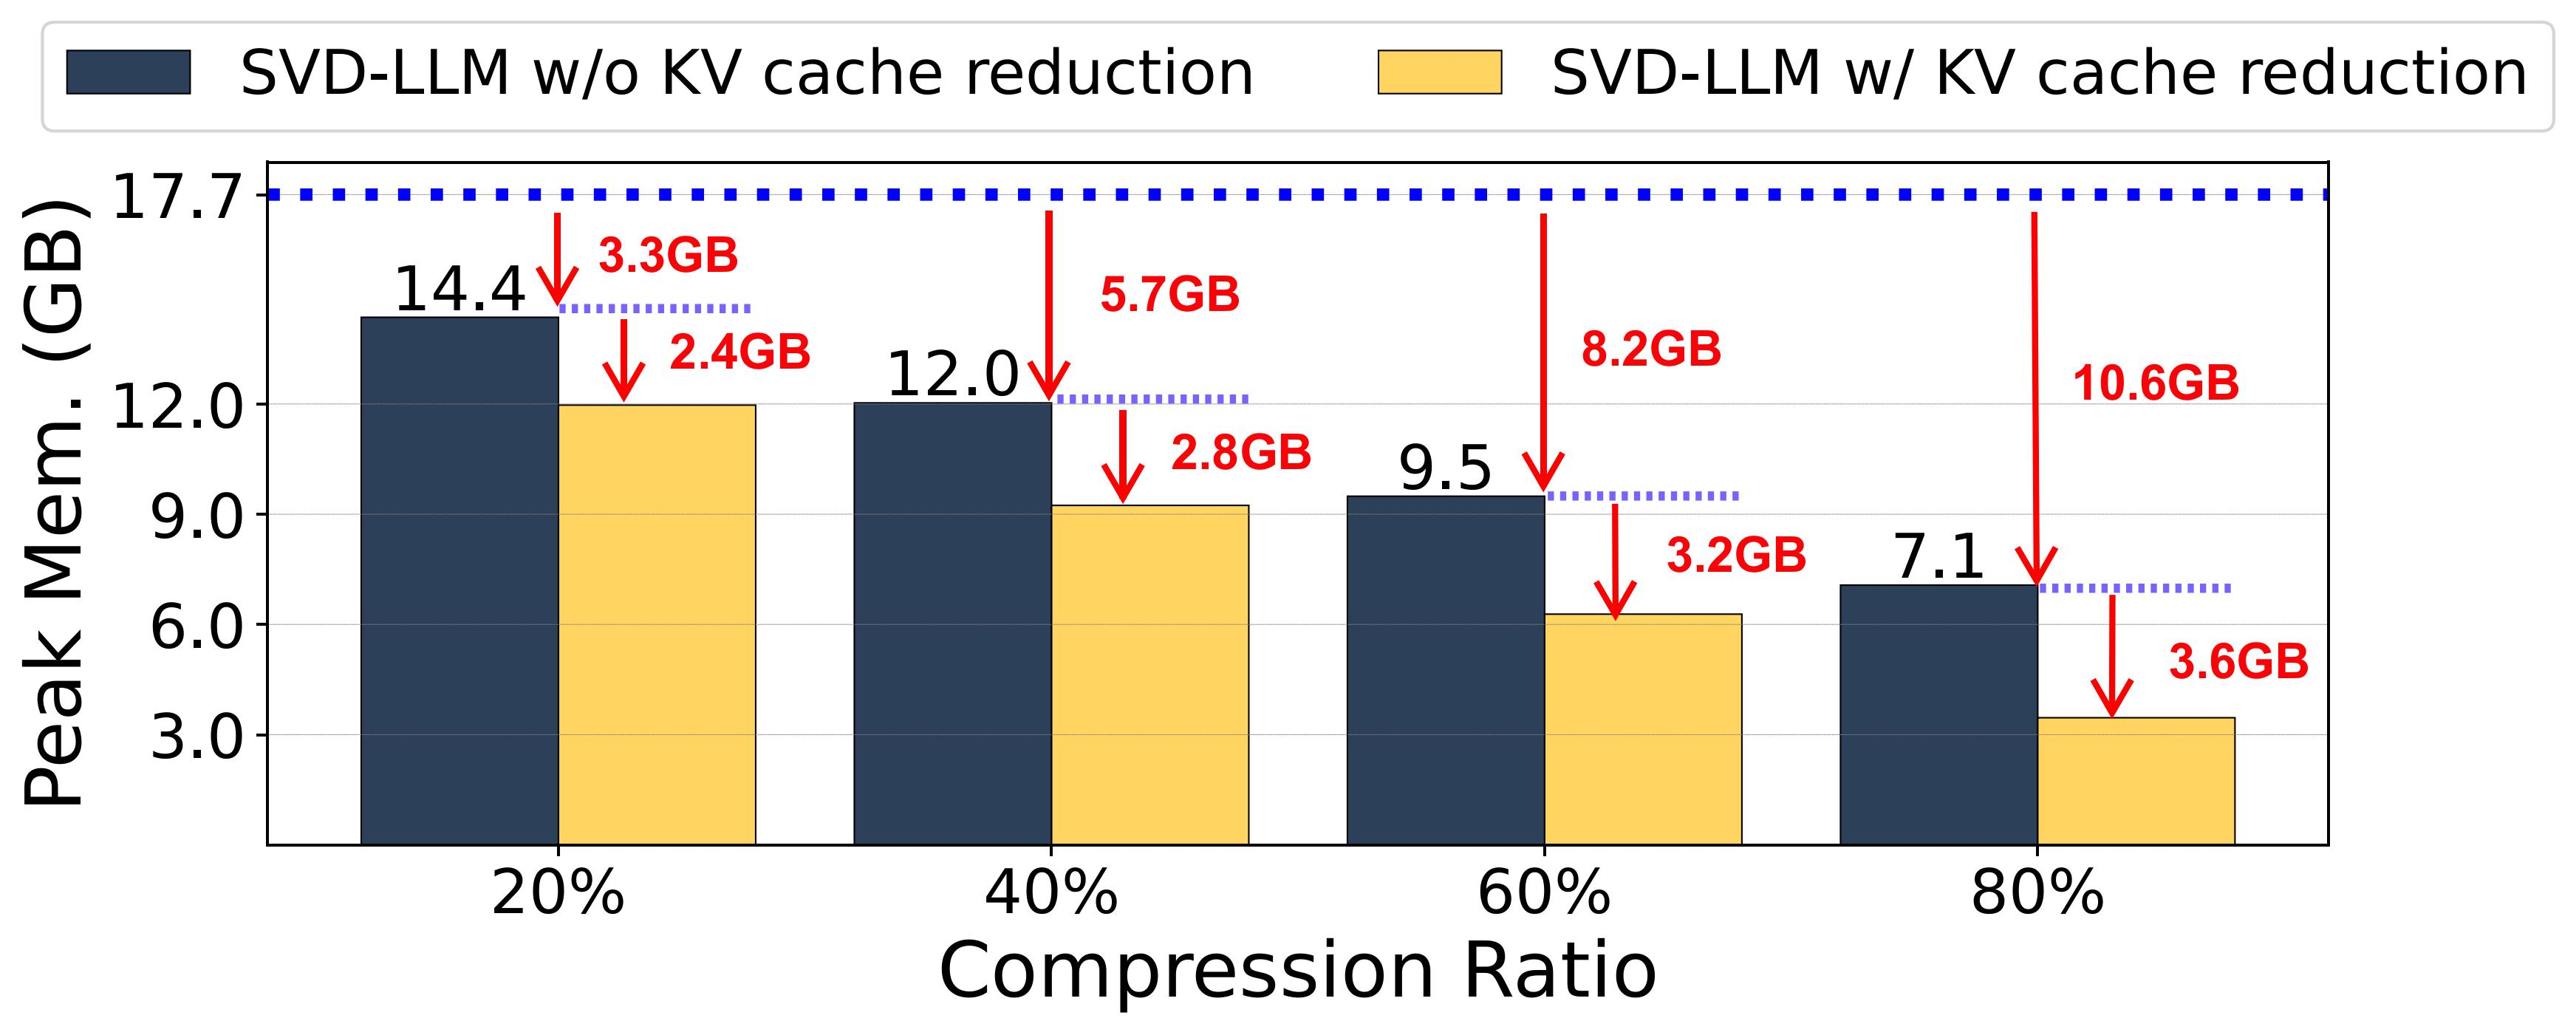
\includegraphics[width=1\textwidth]{Figures/kv_bs_1.jpg}
        \vspace{-5mm}
        \caption{Peak memory to generate 128 tokens with batch size of 32 using LLaMA-7B compressed by \sysname w/ and w/o KV-cache reduction. The dotted line indicates the peak memory of the original LLaMA-7B. The memory reduction from the dotted line to the blue bars mainly comes from the model compression. The memory reduction from the blue to the yellow bars mainly comes from the reduced footprint of the KV cache.}
        \label{fig:kv}
    \end{minipage}%
    \hspace{0.1cm}
    \begin{minipage}{0.485\textwidth}
    \centering
    \sensitivityTable
\end{minipage}
\vspace{-3mm}
\end{figure}

\vspace{-1mm}
\subsection{Ablation Study}
\label{subsec:ablation_study}
\vspace{-1mm}

%\xin{In this section, we provide three ablation studies of \sysname while more are provided in~\cref{appendix:more_ablation} due to page limit.}
%%
% 

\textbf{Modular Sensitivity Study.}
% \vspace{-2mm}
We conduct ablation studies to evaluate the separate contributions of the two key components (i.e., truncation-aware data whitening and parameter update with sequential low-rank approximation) of \sysname. 
%
Let \sysname \texttt{(W)} denote the version of \sysname with truncation-aware data whitening only; \sysname \texttt{(U)} denote the version of \sysname with \xin{normal SVD truncation} and parameter update with sequential low-rank approximation.
%; and \sysname  denote the version of \sysname with both truncation-aware data whitening and parameter update with sequential low-rank approximation.
As shown in~\cref{tab:sensitivity}, we have three observations. 
%
(1) \sysname\texttt{(W)}, \sysname\texttt{(U)} and \sysname  consistently outperform ASVD across all the compression ratios. Notably, when the compression ratio is at and above 40\%, all of them reduce the perplexity by more than 99\% compared to ASVD. 
%
(2) \sysname consistently outperforms both \sysname\texttt{(U)} and \sysname\texttt{(W)} across all compression ratios.
%
This result demonstrates the unique contribution from each of the two key components and the importance of combining both components to achieve the best performance.
%
(3) Comparing between \sysname\texttt{(W)} and \sysname\texttt{(U)}, \sysname\texttt{(W)} achieves a lower perplexity compared to \sysname\texttt{(U)} across all compression ratios. This result indicates that truncation-aware data whitening plays a more significant role than parameter update with sequential
low-rank approximation.
%(3) With the increase of compression ratio, \sysname achieves a much lower perplexity compared to \sysname \texttt{(W)}, highlighting the importance of combining both components in \sysname when the compression ratio increases.

\textbf{Impact of Calibration Data.}
Next, we examine the impact of calibration data on \sysname. 
%
\cref{fig:cali} and~\cref{tab:different_ds_acc} summarize the performance of compressed LLaMA-7B when changing three key characteristics of the calibration data: (1) number of calibration data, (2) the seed used to randomly sample the calibration data, and (3)  dataset from which calibration data is sampled.
% 
As shown, the changes of the three key characteristics on calibration data incur no more than 3\% to the final performance, indicating that the sensitivity of \sysname on calibration data is limited.

\textbf{Impact of Updating Order.}
Lastly, we examine the impact of updating order in the parameter update with sequential low-rank approximation component to the final performance of the compressed LLM. 
%
Table~\ref{tab:lora_acc} shows the performance of compressed LLaMA-7B under 20\% to 80\% compression ratios on WikiText-2 with different updating orders. As shown, there is only a small difference of the final performance between updating matrix $W'_u$ first and updating matrix $W'_v$ first. This result indicates \sysname is not sensitive to the updating order.

More ablation studies are included in~\cref{appendix:more_ablation}.



\begin{figure}[htbp]
\vspace{-4mm}
    \centering
    \begin{minipage}{0.5\textwidth}
    \vspace{2mm}
    \centering
        \subfigure[Change of Number]{
        \centering
        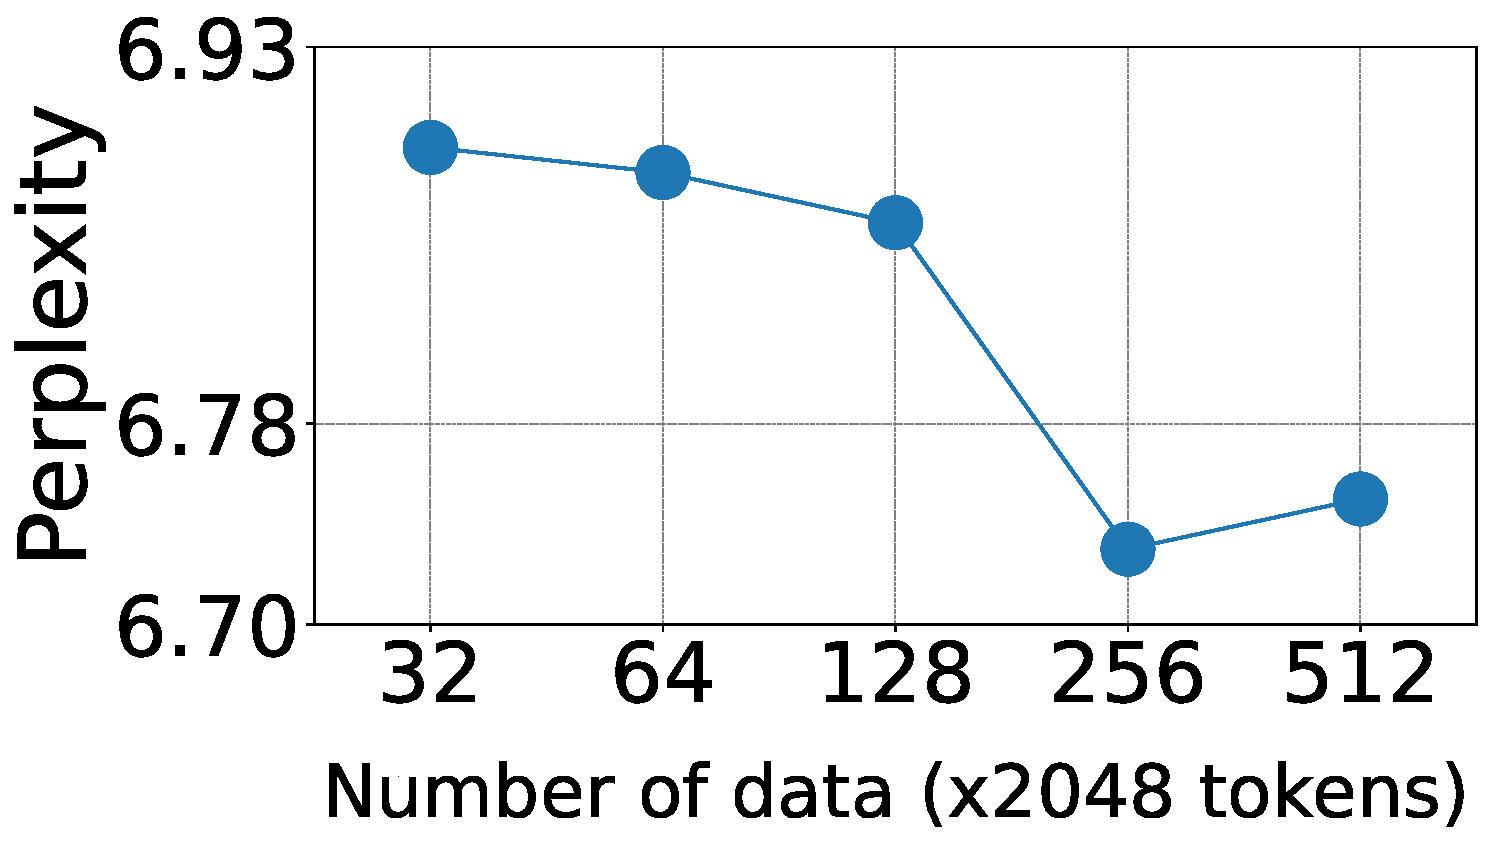
\includegraphics[width=0.455\textwidth]{Figures/cali_size.pdf}
        \label{fig:cali_size}
        }
        \subfigure[Change of Seed]{
        \centering
        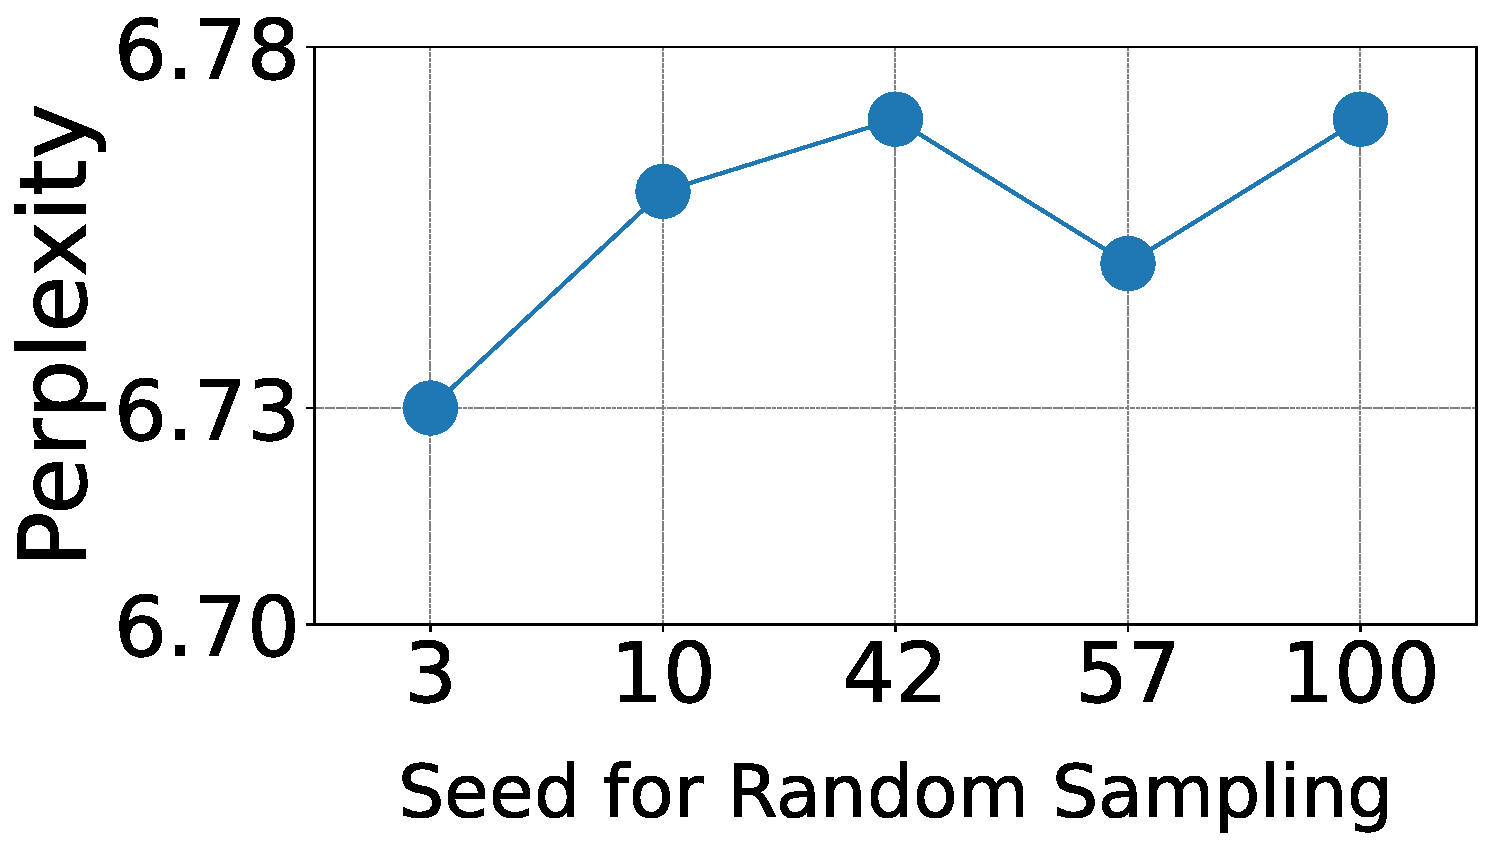
\includegraphics[width=0.45\textwidth]{Figures/seed.pdf}
        \label{fig:seed}
        }
        \vspace{-3mm}
        \DeclareGraphicsExtensions.
        \caption{Perplexity of LLaMA-7B under 20\% compression ratio using calibration data sampled with different number or  seeds from WikiText-2.}
        \label{fig:cali}
        \vspace{6mm}
        \loraTable
    \end{minipage}%
    \hspace{0.1cm}
    \begin{minipage}{0.485\textwidth}
    \vspace{3.5mm}
    \centering
    \datasetTable
\end{minipage}
\vspace{-3mm}
\end{figure}

\begin{figure}[t]
    \centering
    \begin{minipage}{.52\textwidth}
        \svdpruneTable
    \end{minipage}
    \hspace{0.1cm}
    \begin{minipage}{.45\textwidth}
      \svdquantTable
    \end{minipage}%
    % \vspace{-5mm}
\end{figure}


% \vspace{-2mm}
\subsection{Comparison with Other Types of LLM Compression Methods}
\label{subsection:Comparison_with_other_compression_methods}
\vspace{-1mm}
\sysname is orthogonal to other post-training LLM compression methods including pruning and quantization~\citep{DBLP:journals/tmlr/Wan0LA0LQYZZC024, shen2025efficient}. Lastly, we compare the performance of \sysname with state-of-the-art structured pruning-based and quantization-based LLM compression methods. As discussed in Section~\ref{sec:related_works}, since unstructured pruning methods are difficult to achieve its efficiency on hardware, we do not make a comparison with them in this experiment.

\vspace{-0mm}
\textbf{Comparison with Structured Pruning.}
First, we compare \sysname with three state-of-the-art structured pruning-based LLM compression methods: LLM-Pruner~\citep{DBLP:conf/nips/MaFW23}, SliceGPT~\citep{DBLP:conf/iclr/AshkboosCNHH24} and BlockPruner~\citep{DBLP:journals/corr/abs-2406-10594} under the same memory budget, ranging from 10 GB to 7 GB on LLaMA-7B using WikiText-2 dataset. 
%
As shown in Table~\ref{tab:svd_prune}, \sysname outperforms all three structured pruning-based LLM compression methods. In particular, \sysname achieves up to 56\% reduction in perplexity under 7G memory budget.

\vspace{-0mm}
\textbf{Comparison with Quantization.} Finally, we compare \sysname with three state-of-the-art quantization-based LLM compression methods: BiLLM~\citep{DBLP:conf/icml/HuangLQLZ0M024}, PB-LLM~\citep{DBLP:conf/iclr/YuanSD24}, and OneBit~\citep{DBLP:conf/nips/Xu0YWZLLC24}, which push the frontier to 1-bit quantization. 
%
Among them, both BiLLM and PB-LLM are post-training methods, and OneBit is training-required. 
%
The results on LLaMA-7B using WikiText-2 dataset are shown in Table~\ref{tab:svd_quant}. 
%
We have three observations. 
%
(1) Compared to post-training methods PB-LLM and BiLLM, \sysname achieves the best performance. 
%
(2) Training-required method OneBit outperforms \sysname. This result is expected because OneBit involves resource-intensive retraining using large-scale datasets to boost the accuracy after compression. %However, compared to post-training methods such as \sysname which does not require retraining, training-required method is way too expensive.
%
(3) Lastly, we combine \sysname with a 2-bit quantization-based post-training LLM compression method QuIP\#~\citep{DBLP:conf/icml/TsengCSKS24}. This is achieved by first applying \sysname to the LLM under 40\% compression ratio, and then applying QuIP\# for 2-bit quantization on the compressed model ($W'_u$ and $W'_v$) generated from \sysname. As shown in Table~\ref{tab:svd_quant}, \sysname outperforms state-of-the-art 1-bit training-required method OneBit \textit{without} involving resource-intensive retraining. This result demonstrates the potential of a hybrid approach -- integrating SVD-based and quantization-based compression techniques -- to push the boundaries of post-training LLM compression.


%by combining \sysname with a 2-bit quantization-based post-training LLM compression method QuIP\#~\citep{DBLP:conf/icml/TsengCSKS24}\footnote{\xin{This is achieved by first applying SVD-LLM to the LLM under 40\% compression ratio, and then applying QuIP\# for 2-bit quantization on the compressed model generated from SVD-LLM..}}, \sysname outperforms state-of-the-art 1-bit training-required method OneBit without involving resource-intensive retraining,  demonstrating the potential of a hybrid approach—integrating SVD-based and quantization-based compression techniques—to push the boundaries of post-training LLM compression.
%

%This result is important, because it introduces a highly efficient post-training approach that outperforms state-of-the-art 1-bit training-required quantization-based LLM compression method without incurring expensive retraining.